\documentclass[12pt]{article}
\title{Induced universal graphs for families of small graphs}
\author{
        James Trimble \\
                School of Computing Science\\
        University of Glasgow, Glasgow, Scotland \\
        \href{mailto:j.trimble.1@research.gla.ac.uk}{j.trimble.1@research.gla.ac.uk}
}
\date{\today}

\usepackage[letterpaper, total={6in, 8in}]{geometry}
\usepackage[x11names, svgnames, rgb]{xcolor}
\usepackage[utf8]{inputenc}
\usepackage{booktabs}
\usepackage{hyperref}
\usepackage{tikz}
\usepackage{amsthm}
\usetikzlibrary{decorations, decorations.pathreplacing, decorations.pathmorphing,
    calc, backgrounds, positioning, tikzmark, patterns, matrix, fit, graphs,
    snakes, arrows, shapes, calligraphy}
%\usetikzlibrary{snakes,arrows,shapes}
\usepackage{amsmath}
\usepackage{subfigure}
\usepackage{cleveref}
\usepackage[ruled,vlined]{algorithm2e}
\usepackage{algpseudocode}

\usepackage{caption}
\captionsetup{width=0.8\textwidth,font=footnotesize}
%

\crefname{algorithm}{Algorithm}{Algorithms}
\Crefname{algorithm}{Algorithm}{Algorithms}
\crefname{algocf}{Algorithm}{Algorithms}
\Crefname{algocf}{Algorithm}{Algorithms}
\crefname{figure}{Figure}{Figures}
\Crefname{figure}{Figure}{Figures}
\crefname{table}{Table}{Tables}
\Crefname{table}{Table}{Tables}
\crefname{section}{Section}{Sections}
\Crefname{section}{Section}{Sections}

\newcommand{\calF}{\ensuremath{\mathcal{F}}}
\newcommand{\calG}{\ensuremath{\mathcal{G}}}
\newcommand{\AlgVar}[1]{\mathit{#1}}

\newcommand{\lineref}[1]{line~\ref{#1}}
\newcommand{\codelineref}[1]{line~\ref{#1}}
\newcommand{\linerangeref}[2]{lines~\ref{#1} to~\ref{#2}}
\newcommand{\Lineref}[1]{Line~\ref{#1}}
\newcommand{\Linerangeref}[2]{Lines~\ref{#1} to~\ref{#2}}

% https://tex.stackexchange.com/a/184829
\algnewcommand{\LeftComment}[1]{\(\triangleright\) #1}

\newtheorem{proposition}{Proposition}

\definecolor{uofguniversityblue}{rgb}{0, 0.219608, 0.396078}

\definecolor{uofgheather}{rgb}{0.356863, 0.32549, 0.490196}
\definecolor{uofgaquamarine}{rgb}{0.603922, 0.72549, 0.678431}
\definecolor{uofgslate}{rgb}{0.309804, 0.34902, 0.380392}
\definecolor{uofgrose}{rgb}{0.823529, 0.470588, 0.709804}
\definecolor{uofgmocha}{rgb}{0.709804, 0.564706, 0.47451}

\definecolor{uofglawn}{rgb}{0.517647, 0.741176, 0}
\definecolor{uofgcobalt}{rgb}{0, 0.615686, 0.92549}
\definecolor{uofgturquoise}{rgb}{0, 0.709804, 0.819608}
\definecolor{uofgsunshine}{rgb}{1.0, 0.862745, 0.211765}
\definecolor{uofgpumpkin}{rgb}{1.0, 0.72549, 0.282353}
\definecolor{uofgthistle}{rgb}{0.584314, 0.070588, 0.447059}
\definecolor{uofgpillarbox}{rgb}{0.701961, 0.047059, 0}
\definecolor{uofglavendar}{rgb}{0.356863, 0.301961, 0.580392}

\definecolor{uofgsandstone}{rgb}{0.321569, 0.278431, 0.231373}
\definecolor{uofgforest}{rgb}{0, 0.317647, 0.2}
\definecolor{uofgburgundy}{rgb}{0.490196, 0.133333, 0.223529}
\definecolor{uofgrust}{rgb}{0.603922, 0.227451, 0.023529}

\begin{document}

\maketitle
%
\begin{abstract}
For $0 \leq k \leq 6$, we give the minimum number of vertices $f(k)$ in a graph containing all
$k$-vertex graphs as induced subgraphs, and show
that $16 \leq f(7) \leq 18$.  For $0 \leq k \leq 5$, we also give the counts of
such graphs, as generated by brute-force computer search.  We give additional
results for small graphs containing all trees on $k$ vertices.
\end{abstract}

\section{Introduction}

Given a collection $\calF$ of graphs, graph $G$ is \emph{induced universal} for
$\calF$ if and only if each element of $\calF$ is an induced subgraph of $G$.
Graph $G$ is a \emph{minimal} induced universal graph for $\calF$ if it has as
few vertices as possible.  The problem of finding a minimal induced universal graph
of a family of graphs generalises the minimum common supergraph problem
\cite{DBLP:journals/computing/BunkeJK00}.

We write $\calF(k)$ to denote the family of all graphs on $k$ vertices,
and we write $f(k)$ to denote the order (that is, the
number of vertices) of a minimal induced universal graph for $\calF(k)$.
We write $F(k)$ to denote the number of non-isomorphic graphs of order $f(k)$
that are induced universal for $f(k)$.
To give an example, we have $f(3)=5$ and $F(3)=5$. All five of the minimal induced universal graphs
for $\calF(3)$ are shown in \Cref{fig:univ3a}. \Cref{fig:univ3b} shows the four
graphs in $\calF(3)$ as induced subgraphs of a single induced universal graph.

Moon showed that $f(k) \leq 2^{(k-1)/2}$
\cite{moon_1965}, and Alon showed that $f(k) = (1 + o(1))2^{(k-1)/2}$
\cite{alon2017asymptotically}.  There is an extensive literature on bounds on
the order of minimal induced universal subgraphs for many families of graphs;
see the references in \cite{alon2017asymptotically}.
However, to my knowledge the only
existing systematic attempt to find \emph{exact} values for families of small
graphs is an answer by James Preen on the Mathematics Stack Exchange website that
presents results for families of small connected graphs obtained by brute-force
search with the Maple programming language \cite{preen_math_se}.

\begin{figure}[htb]
    \centering

    \subfigure[][The five induced universal graphs of order 5 for \calF(3) (that is, for the family of all 3-vertex graphs)] {
      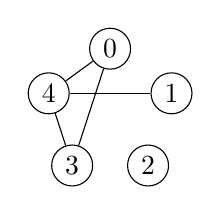
\begin{tikzpicture}[>=latex',line join=bevel,scale=.4]
        \graph [nodes={draw, circle, minimum width=.52cm, inner sep=1pt}, circular placement, radius=0.82cm,
                clockwise=5] {
                    0,1,2,3,4;
           3 -- 0;
           4 -- 0;
           4 -- 1;
           4 -- 3;
        };
      \end{tikzpicture}
      \qquad
      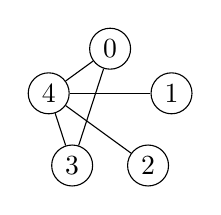
\begin{tikzpicture}[>=latex',line join=bevel,scale=.4]
        \graph [nodes={draw, circle, minimum width=.52cm, inner sep=1pt}, circular placement, radius=0.82cm,
                clockwise=5] {
                    0,1,2,3,4;
          3 -- 0;
          4 -- 0;
          4 -- 1;
          4 -- 2;
          4 -- 3;
        };
      \end{tikzpicture}
      \qquad
      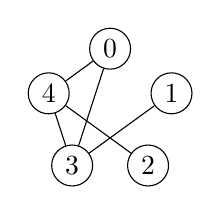
\begin{tikzpicture}[>=latex',line join=bevel,scale=.4]
        \graph [nodes={draw, circle, minimum width=.52cm, inner sep=1pt}, circular placement, radius=0.82cm,
                clockwise=5] {
                    0,1,2,3,4;
          3 -- 0;
          3 -- 1;
          4 -- 0;
          4 -- 2;
          4 -- 3;
        };
      \end{tikzpicture}
      \qquad
      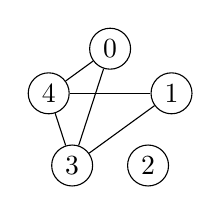
\begin{tikzpicture}[>=latex',line join=bevel,scale=.4]
        \graph [nodes={draw, circle, minimum width=.52cm, inner sep=1pt}, circular placement, radius=0.82cm,
                clockwise=5] {
                    0,1,2,3,4;
          3 -- 0;
          3 -- 1;
          4 -- 0;
          4 -- 1;
          4 -- 3;
        };
      \end{tikzpicture}
      \qquad
      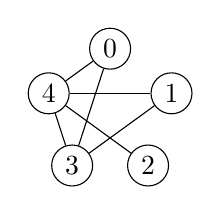
\begin{tikzpicture}[>=latex',line join=bevel,scale=.4]
        \graph [nodes={draw, circle, minimum width=.52cm, inner sep=1pt}, circular placement, radius=0.82cm,
                clockwise=5] {
                    0,1,2,3,4;
          3 -- 0;
          3 -- 1;
          4 -- 0;
          4 -- 1;
          4 -- 2;
          4 -- 3;
        };
      \end{tikzpicture}
      \label{fig:univ3a}
    }

    \par\bigskip
    \subfigure[][A demonstration that the first graph in \Cref{fig:univ3a} is induced universal
            for $\calF(3)$.  For each graph $G$ in $\calF(3)$ ($I_3$, $K_3$, $P_3$, and
            a graph with a single edge), an induced subgraph isomorphic to $G$ is shown in a
            single color.] {
      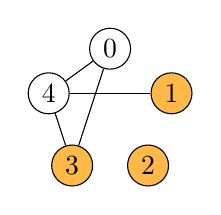
\begin{tikzpicture}[>=latex',line join=bevel,scale=.4]
        \graph [nodes={draw, circle, minimum width=.52cm, inner sep=1pt}, circular placement, radius=0.82cm,
                clockwise=5] {
                    0,1[fill=uofgpumpkin],2[fill=uofgpumpkin],3[fill=uofgpumpkin],4;
           3 -- 0;
           4 -- 0;
           4 -- 1;
           4 -- 3;
        };
      \end{tikzpicture}
      \qquad
      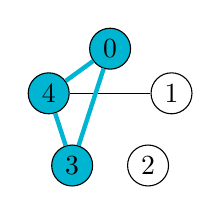
\begin{tikzpicture}[>=latex',line join=bevel,scale=.4]
        \graph [nodes={draw, circle, minimum width=.52cm, inner sep=1pt}, circular placement, radius=0.82cm,
                clockwise=5] {
                    0[fill=uofgturquoise],1,2,3[fill=uofgturquoise],4[fill=uofgturquoise];
           4 -- 1;
           3 --[uofgturquoise, ultra thick] 0;
           4 --[uofgturquoise, ultra thick] 0;
           4 --[uofgturquoise, ultra thick] 3;
        };
      \end{tikzpicture}
      \qquad
      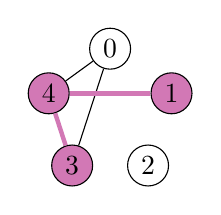
\begin{tikzpicture}[>=latex',line join=bevel,scale=.4]
        \graph [nodes={draw, circle, minimum width=.52cm, inner sep=1pt}, circular placement, radius=0.82cm,
                clockwise=5] {
                    0,1[fill=uofgrose],2,3[fill=uofgrose],4[fill=uofgrose];
           3 -- 0;
           4 -- 0;
           4 --[uofgrose, ultra thick] 1;
           4 --[uofgrose, ultra thick] 3;
        };
      \end{tikzpicture}
      \qquad
      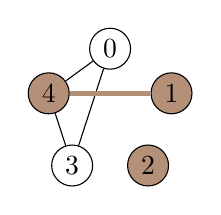
\begin{tikzpicture}[>=latex',line join=bevel,scale=.4]
        \graph [nodes={draw, circle, minimum width=.52cm, inner sep=1pt}, circular placement, radius=0.82cm,
                clockwise=5] {
                    0,1[fill=uofgmocha],2[fill=uofgmocha],3,4[fill=uofgmocha];
           3 -- 0;
           4 -- 0;
           4 --[uofgmocha, ultra thick] 1;
           4 -- 3;
        };
      \end{tikzpicture}
      \label{fig:univ3b}
    }
\caption{Induced universal graphs for the family of all graphs on 3 vertices}
\label{fig:graphs}
\end{figure}

This paper uses a brute-force approach similar to that of Preen to find minimal
induced universal graphs for families of small \emph{general} graphs.
Section~\ref{sec:method} describes our computer search method, including an
optimisation to reduce run times.  Sections~\ref{sec:results5} presents exact
values of $f(k)$ for $k \leq 5$ along with
the corresponding counts of minimal induced universal subgraphs.
Section~\ref{sec:f6} gives the value of $f(6)$ and and
Section~\ref{sec:f7} gives bounds on $f(7)$; in each of these sections, the lower
bound is proven and a graph obtained by heuristic search demonstrating the
upper bound is given.  Finally, Section~\ref{sec:trees} gives results for
families of trees.

\section{Generating all induced universal graphs}\label{sec:method}

Given $\calF$ and $n$,
we use the brute-force approach described by Preen \cite{preen_math_se} and shown
in \Cref{alg:brute-force} to find the set of
$n$-vertex graphs that are induced universal for the family $\calF$.
The function $\FuncSty{AllInducedUniversalGraphs}()$ is the entry point.
\Lineref{TryEachG} tests in turn each candidate graph $G$ from the family
of $n$-vertex graphs, and adds to the collection $\calG$ those that are induced universal
for $\calF$.  The function $\FuncSty{IsInducedUniversal}()$ tests
whether a graph $G$ is induced universal for $\calF$ by checking that
$H$ is isomorphic to a subgraph of $G$ for each $G \in \calF$.

For the collection $\calF(n)$ of candidate graphs on \lineref{TryEachG}, our
implementation uses Brendan McKay's lists of
graphs\footnote{\url{https://users.cecs.anu.edu.au/~bdm/data/graphs.html}}.
These are read in \texttt{graph6}
format\footnote{\url{https://users.cecs.anu.edu.au/~bdm/data/formats.html}}
from a text file as the program proceeds, and therefore only one candidate
graph at a time needs to be stored in memory.

For the call $\FuncSty{InducedSubIso}()$ to an algorithm for the induced
subgraph isomorphism decision problem on line \lineref{CallSubIso},
our program uses a Python implementation of the McSplit
algorithm \cite{DBLP:conf/ijcai/McCreeshPT17}.
McSplit was designed for
the more general maximum common induced subgraph problem,
but it can be used for induced subgraph isomorphism with a simple
modification: we backtrack when the calculated upper bound
on the order of a common subgraph is less the order of graph $H$.
This method for solving
the subgraph isomorphism problem is very fast if both input graphs
are small, as the graphs considered in this paper are.
While McSplit is suitable for our purposes in this paper,
we do not claim that it is the the fastest induced subgraph isomorphism
solver for very small graphs; it would be useful future work to perform
an experimental comparison with other subgraph isomorphism solvers.
%%% (Although
%%% I have described the application of this method to families of all graphs of a given order,
%%% the method could easily be applied to any family $\calF$ of graphs, and indeed
%%% Section~\ref{sec:trees} gives results from the application of this method
%%% to families of trees.)

\begin{algorithm}[h!]
\DontPrintSemicolon
%%% \nl $\FuncSty{Search}(\AlgVar{future},M)$ \;
%%% \nl \Begin{
%%% %\nl \lIf {$\AlgVar{future} = \emptyset$ \bf{and} $|M| > |\AlgVar{incumbent}|$}
%%% \nl \lIf {$|M| > |\AlgVar{incumbent}|$}{$\AlgVar{incumbent} \gets M$} \label{StoreIncumbent}
%%% %\nl \lIf {$\AlgVar{future} = \emptyset$}{return}
%%% \medskip
%%% \nl $\AlgVar{bound} \gets |M|  + \sum_{\langle \setG,\setH \rangle \in \AlgVar{future}} \min(|\setG|,|\setH|)$ \label{CalcBound} \;
%%% \nl \lIf {$\AlgVar{bound} \leq |\AlgVar{incumbent}|$}{\KwSty{return}} \label{PruneSearch}
%%% \medskip
%%% \nl $\langle \setG,\setH \rangle \gets \FuncSty{SelectLabelClass}(\AlgVar{future})$ \label{SelectClass} \;
%%% \nl $v \gets \FuncSty{SelectVertex}(\setG)$ \label{SelectVertex} \;
%%% \nl \For {$w \in \setH$ \label{WLoop}} {
%%% \nl    $\AlgVar{future'} \gets \emptyset$ \label{NewFuture} \;
%%% \nl    \For {$\langle \setG',\setH'\rangle \in future$ \label{InnerLoop}}{
%%% \nl        $\setG'' \gets \setG' \cap \N(\graphG, v) \setminus \{v\}$ \label{NewPWithEdge} \;
%%% \nl        $\setH'' \gets \setH' \cap \N(\graphH, w) \setminus \{w\}$ \;
%%% \nl        \If {$\setG'' \neq \emptyset$ \bf{and} $\setH'' \neq \emptyset$\label{IfNonEmpty}}{
%%% \nl            $\AlgVar{future'} \gets \AlgVar{future'} \cup \{\langle \setG'' , \setH'' \rangle\}$ \label{AddToFutureWithEdge}}
%%% \nl        $\setG'' \gets \setG' \cap \invN(\graphG, v) \setminus \{v\}$ \label{NewPWithoutEdge}  \;
%%% \nl        $\setH'' \gets \setH' \cap \invN(\graphH, w) \setminus \{w\}$ \;
%%% \nl        \If {$\setG'' \neq \emptyset$ \bf{and} $\setH'' \neq \emptyset$\label{IfNonEmpty2}}{
%%% \nl            $\AlgVar{future'} \gets \AlgVar{future'} \cup \{\langle \setG'' , \setH'' \rangle\}$} \label{InnerLoopEnd}
%%%        }
%%% \nl   $\FuncSty{Search}(\AlgVar{future'},M\cup \{(v,w)\})$ \label{ExpandWithV} \;
%%%   }
%%% \nl $\setG' \gets \setG \setminus \{v\}$ \label{RemoveV} \;
%%% \nl $\AlgVar{future} \gets \AlgVar{future} \setminus \{\langle \setG,\setH \rangle\}$\;
%%% \nl \lIf {$\setG' \neq \emptyset$} {$\AlgVar{future} \gets \AlgVar{future} \cup \{\langle \setG',\setH \rangle \}$}
%%% \nl $\FuncSty{Search}(\AlgVar{future},M)$ \label{ExpandWithoutV} \;
%%% }
%%% \;
\nl $\FuncSty{IsInducedUniversal}(\calF,G)$ \label{BruteForceFun} \;
\nl \KwData{A family of graphs $\calF$ and a graph $G$.}
\nl \KwResult{A logical value indicating whether $G$ is induced universal for $\calF$.}
\nl \Begin{
\nl    \For {$H \in \calF$ \label{HLoop}}{
\nl      \lIf {$\neg\FuncSty{InducedSubIso}(H, G)$\label{CallSubIso}}{$\KwSty{return}$~$\AlgVar{false}$}
       }
\nl   $\KwSty{return}$~$\AlgVar{true}$ \;
    }
\medskip
\nl $\FuncSty{AllInducedUniversalGraphs}(\calF,n)$ \label{BruteForceFun} \;
\nl \KwData{A family of graphs $\calF$ and a natural number $n$.}
\nl \KwResult{The set of all graphs of order $n$ that are induced universal for $\calF$.}
\nl \Begin{
\nl    $\calG \gets \emptyset$ \;
\nl    \For {$G \in \calF(n)$}{
\nl      \lIf {$\FuncSty{IsInducedUniversal}(\calF,G)$\label{TryEachG}}{$\calG \gets \calG \cup \{G\}$}
       }
\nl   $\KwSty{return}$~$\calG$ \;
    }
\caption{A brute-force algorithm for finding all order-$n$ induced universal subgraphs of a family $\calF$ of graphs.
	The entry point is $\FuncSty{AllInducedUniversalGraphs}(\calF,n)$.}
\label{alg:brute-force}
\end{algorithm}

The full set of experiments described in this paper, run sequentially,
took less than an hour to complete on a laptop with an Intel Core i5-6200U CPU
and 8 GB RAM.\footnote{The code and
results from this paper, including lists of minimal induced universal graphs
in graph6 format, are available from
\url{https://github.com/jamestrimble/small-universal-graphs}}

\section{Iteration order for $\calF$}\label{sec:iteration-order}

When deciding on \lineref{HLoop} of the algorithm whether a graph $G$ contains
every element of $\calF$ as an induced subgraph, are some iteration orders of
$\calF$ better than others?  For a graph $G$ that contains a copy of each
element of $\calF$, the iteration order is of no importance; we much check
every element of $\calF$ before returning $\AlgVar{true}$.  For a graph $G$ that
does \emph{not} contain a copy of each element of $\calF$, however, we would like
to iterate over $\calF$ in an order such that graphs that are likely to fail the
subgraph isomorphism test are checked early; that way, we can quickly return
$\AlgVar{false}$.

We begin by considering the case where $\calF = \calF(k)$ for some $k$; that is,
$\calF$ is the set of all graphs of order $k$.
As Diaconis and Chatterjee note, \cite{chatterjee2021isomorphisms}, the complete
graph $K_n$ is the `hardest' graph of order $n$ for a random graph to contain.
This led me
to consider two possible orderings in which $K_k$ and its complement $I_k$ come
first.  The first of these approaches is to the sort $\calF(k)$ such that
graphs with large automorphism groups appear first.  (Intuitively, if a graph
has few automorphisms then we can generate many different labelled graphs
by permuting the vertex labels.  This gives more `opportunities' for the
graph to be an induced subgraph of $G$.)
The second approach considered is to place graphs
with unusually high or low edge counts, as measured by the absolute value of
${2|E(G)| - {|V(G)| \choose 2}}$, first.

\Cref{fig:scatter} examines whether graphs that appear early in the orderings
of $\calF$
generated by each of these two strategies are contained in few graphs with
a given number of vertices, as we would hope to be the case.
For this experiment, we let $\calF = \calF(5)$, and we consider the problem
of finding induced universal graphs of order 8.
Each point on the plots
represents one of the 34 graphs of order 5 (fewer than 34 points are visible
due to exactly-overlapping points, as we would expect).  On the vertical
axis, we have the number of graphs in $\calF(8)$ containing $G$; we would like
graphs for which this value is small to appear early in our order.
On the horizontal axes we have each of our two measures: size of automorphism group
and `extremeness' of edge count.  The first of these measures has a strong correlation
with the number of graphs containing $G$ as an induced subgraph, suggesting that
it is a good strategy to use when sorting the list of graphs.

\begin{figure}[htb]
    \centering

%    \subfigure[][TODO caption] {
      \includegraphics*{img/automorphisms-scatter.pdf}
%      \label{fig:scatter-a}
%    }
     \qquad
%    \subfigure[][TODO caption] {
      \includegraphics*{img/deg-scatter.pdf}
%      \label{fig:scatter-b}
%    }
    \caption{For each graph $G \in \calF(5)$, we plot on the vertical axis
    the number of graphs in $\calF(8)$ that contain $G$ as an induced subgraph.
    This value has a strong negative correlation with the size of the automorphism
    group of $G$ (left plot), but a weaker correlation with a measure of how
    extreme the edge count of $G$ is (right plot).
    All axis scales are logarithmic.}
\label{fig:scatter}
\end{figure}

\subsection{Testing the strategies: $\calF = \calF{5}$}

We now test whether each of our ordering strategies results, as hoped,
in a reduced number of calls to the subgraph isomorphism function
in \Cref{alg:brute-force}.  As our first test case, we consider 
$\FuncSty{AllInducedUniversalGraphs}(\calF(5),9)$ ---
finding all induced universal graphs of order 9 for the family of
all graphs of order 5.  We consider four strategies.
The first two of these are the automorphism-count and `degree extremeness'
measures described above.  The fourth strategy is a random order.
Finally, we used one further strategy, which we call ``almost random''.
Under this strategy, $I_5$ and $K_5$ are placed at the start of the list,
and the remaining 32 graphs are in random order.  This strategy was not
intended to be useful in practice, but to give insight into whether
the success of the first two strategies was purely due to having
$I_5$ and $K_5$ at the start of the list of graphs.
For each of these strategies, we ran the program 50 times.

The results are shown in \Cref{fig:second-experiment}.  Over 50 runs,
the `automorphisms` strategy required a mean of 304,758 calls to the subgraph
isomorphism solver, while the `degree' strategy required a very similar
number of calls:  a mean of 304,701.  Surprisingly, the `almost random'
strategy had the lowest average number of calls of all the strategies,
at 304,431.  The `random' strategy fared poorly, requiring 822,649
calls on average and a minimum of 451,287 calls in the best of the 50 runs.
The variance in number of calls was tiny for all but the random strategy,
with between 304,000 and 305,000 calls being required for each run.

We note, first, that `degree' strategy appears to be at least as effective
as the `automorphisms' strategy for this instance, despite the lower
correlation observed in \Cref{fig:scatter}.  Perhaps most surprising is
that the `almost random' strategy performed better than any of the other
strategies.

\begin{figure}[htb]
    \centering

    \includegraphics*[width=0.7\textwidth]{img/second-experiment-plot}

    \caption{TODO}
\label{fig:second-experiment}
\end{figure}

\subsection{Testing the strategies: $\calF \subset \calF{5}$}

TODO abcdef

\begin{figure}[htb]
    \centering

    \includegraphics*[width=0.7\textwidth]{img/second-experiment-plot-using-sample}

    \caption{TODO}
\label{fig:second-experiment-using-sample}
\end{figure}

\section{Results for \texorpdfstring{$k \leq 5$}{k<=5}}\label{sec:results5}

Table~\ref{tab:graphresults} shows, for $0 \leq k \leq 5$, the value of $f(k)$.
The table also shows $F(k)$, the number of minimal induced universal
graphs for the family of all $k$-vertex graphs.  To my knowledge, the value of
$f(5)$ and the values of $F(k)$ have not been published previously.

The values $f(1)$, $f(2)$ and $f(3)$ are equal to to the simple lower bound $2k
- 1$ given in a question by ``Chain Markov'' on Mathematics Stack Exchange
  \cite{math_se_question}.  The values $f(4)$ and $f(5)$ are equal to a lower
  bound given in a comment by ``bof'' on the same question: $f(k) \geq 2k$ if $k
  \geq 4$.  (For $k < 10$, this bound improves upon Moon's lower bound $f(k)
  \leq 2^{(k-1)/2}$.) To briefly summarise the proof, if $f(k) \leq 2k$ then $G$
  must be a split graph (that is, a graph whose vertices can be partitioned
  into a clique and an independent set); therefore, $G$ cannot contain the
  cycle $C_4$ as an induced subgraph.  An example of an 8-vertex induced
  universal graph for the family of 4-vertex graphs was given by ``Chain
  Markov'' as a comment on the same question.

\begin{table}[h!]
\centering
\begin{tabular}{r r r}
 \toprule
 $k$ & $f(k)$ & $F(k)$ \\ [0.5ex]
 \midrule
 0 & 0 & 1 \\
 1 & 1 & 1 \\
 2 & 3 & 2 \\
 3 & 5 & 5 \\
 4 & 8 & 438 \\
 5 & 10 & 22 \\
 \bottomrule
\end{tabular}
\caption{For each $k$, $f(k)$ is the minimum order of a graph containing all $k$-vertex graphs as
induced subgraphs, and $F(k)$ is the number of distinct $f(k)$-vertex graphs that contain
all $k$-vertex graphs as induced subgraphs.}
\label{tab:graphresults}
\end{table}
%
%

Figure~\ref{fig:graphs} shows examples of minimal induced universal graphs
for the families of all graphs with three, four and five vertices
respectively.

\begin{figure}[htb]
    \centering

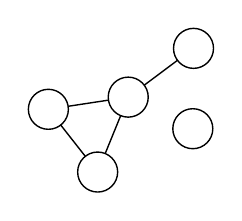
\begin{tikzpicture}[>=latex',line join=bevel,scale=.4]
  \pgfsetlinewidth{.5bp}
%%
\pgfsetcolor{black}
  % Edge: 3 -- 0
  \draw [] (51.166bp,32.248bp) .. controls (44.492bp,40.742bp) and (36.044bp,51.496bp)  .. (29.344bp,60.024bp);
  % Edge: 4 -- 0
  \draw [] (71.737bp,82.653bp) .. controls (60.758bp,80.98bp) and (46.814bp,78.855bp)  .. (35.882bp,77.189bp);
  % Edge: 4 -- 1
  \draw [] (104.4bp,96.268bp) .. controls (113.37bp,102.97bp) and (124.85bp,111.55bp)  .. (133.86bp,118.28bp);
  % Edge: 4 -- 3
  \draw [] (82.931bp,68.405bp) .. controls (78.728bp,58.107bp) and (73.39bp,45.028bp)  .. (69.205bp,34.773bp);
  % Node: 0
\begin{scope}
  \definecolor{strokecol}{rgb}{0.0,0.0,0.0};
  \pgfsetstrokecolor{strokecol}
  \draw (18.0bp,74.46bp) ellipse (18.0bp and 18.0bp);
\end{scope}
  % Node: 1
\begin{scope}
  \definecolor{strokecol}{rgb}{0.0,0.0,0.0};
  \pgfsetstrokecolor{strokecol}
  \draw (148.63bp,129.31bp) ellipse (18.0bp and 18.0bp);
\end{scope}
  % Node: 2
\begin{scope}
  \definecolor{strokecol}{rgb}{0.0,0.0,0.0};
  \pgfsetstrokecolor{strokecol}
  \draw (148.0bp,57.0bp) ellipse (18.0bp and 18.0bp);
\end{scope}
  % Node: 3
\begin{scope}
  \definecolor{strokecol}{rgb}{0.0,0.0,0.0};
  \pgfsetstrokecolor{strokecol}
  \draw (62.36bp,18.0bp) ellipse (18.0bp and 18.0bp);
\end{scope}
  % Node: 4
\begin{scope}
  \definecolor{strokecol}{rgb}{0.0,0.0,0.0};
  \pgfsetstrokecolor{strokecol}
  \draw (89.87bp,85.42bp) ellipse (18.0bp and 18.0bp);
\end{scope}
%
\end{tikzpicture}
\qquad
\qquad
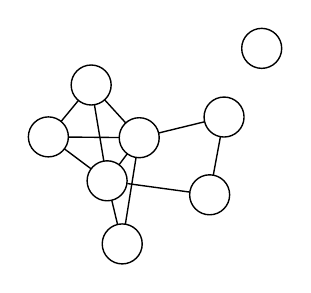
\begin{tikzpicture}[>=latex',line join=bevel,scale=.4]
  \pgfsetlinewidth{.5bp}
%%
\pgfsetcolor{black}
  % Edge: 4 -- 0
  \draw [] (44.956bp,147.01bp) .. controls (40.082bp,141.1bp) and (34.42bp,134.24bp)  .. (29.546bp,128.33bp);
  % Edge: 5 -- 1
  \draw [] (166.49bp,80.229bp) .. controls (168.44bp,90.759bp) and (170.89bp,103.99bp)  .. (172.84bp,114.47bp);
  % Edge: 6 -- 0
  \draw [] (81.617bp,113.74bp) .. controls (68.067bp,113.87bp) and (49.632bp,114.04bp)  .. (36.095bp,114.17bp);
  % Edge: 6 -- 1
  \draw [] (117.47bp,117.89bp) .. controls (129.81bp,120.9bp) and (146.19bp,124.9bp)  .. (158.51bp,127.9bp);
  % Edge: 6 -- 2
  \draw [] (96.884bp,95.599bp) .. controls (94.148bp,78.511bp) and (90.056bp,52.957bp)  .. (87.325bp,35.896bp);
  % Edge: 6 -- 4
  \draw [] (87.484bp,127.04bp) .. controls (81.59bp,133.51bp) and (74.549bp,141.23bp)  .. (68.67bp,147.68bp);
  % Edge: 7 -- 0
  \draw [] (56.422bp,85.611bp) .. controls (48.962bp,91.188bp) and (39.886bp,97.973bp)  .. (32.429bp,103.55bp);
  % Edge: 7 -- 2
  \draw [] (75.094bp,57.147bp) .. controls (76.715bp,50.372bp) and (78.564bp,42.641bp)  .. (80.189bp,35.849bp);
  % Edge: 7 -- 4
  \draw [] (67.894bp,92.673bp) .. controls (65.43bp,107.47bp) and (61.945bp,128.39bp)  .. (59.482bp,143.18bp);
  % Edge: 7 -- 5
  \draw [] (89.1bp,72.32bp) .. controls (105.38bp,70.096bp) and (129.09bp,66.857bp)  .. (145.27bp,64.648bp);
  % Edge: 7 -- 6
  \draw [] (81.628bp,89.246bp) .. controls (84.002bp,92.431bp) and (86.52bp,95.808bp)  .. (88.898bp,99.0bp);
  % Node: 0
\begin{scope}
  \definecolor{strokecol}{rgb}{0.0,0.0,0.0};
  \pgfsetstrokecolor{strokecol}
  \draw (18.0bp,114.33bp) ellipse (18.0bp and 18.0bp);
\end{scope}
  % Node: 1
\begin{scope}
  \definecolor{strokecol}{rgb}{0.0,0.0,0.0};
  \pgfsetstrokecolor{strokecol}
  \draw (176.12bp,132.19bp) ellipse (18.0bp and 18.0bp);
\end{scope}
  % Node: 2
\begin{scope}
  \definecolor{strokecol}{rgb}{0.0,0.0,0.0};
  \pgfsetstrokecolor{strokecol}
  \draw (84.46bp,18.0bp) ellipse (18.0bp and 18.0bp);
\end{scope}
  % Node: 3
\begin{scope}
  \definecolor{strokecol}{rgb}{0.0,0.0,0.0};
  \pgfsetstrokecolor{strokecol}
  \draw (210.0bp,194.0bp) ellipse (18.0bp and 18.0bp);
\end{scope}
  % Node: 4
\begin{scope}
  \definecolor{strokecol}{rgb}{0.0,0.0,0.0};
  \pgfsetstrokecolor{strokecol}
  \draw (56.51bp,161.02bp) ellipse (18.0bp and 18.0bp);
\end{scope}
  % Node: 5
\begin{scope}
  \definecolor{strokecol}{rgb}{0.0,0.0,0.0};
  \pgfsetstrokecolor{strokecol}
  \draw (163.15bp,62.21bp) ellipse (18.0bp and 18.0bp);
\end{scope}
  % Node: 6
\begin{scope}
  \definecolor{strokecol}{rgb}{0.0,0.0,0.0};
  \pgfsetstrokecolor{strokecol}
  \draw (99.76bp,113.58bp) ellipse (18.0bp and 18.0bp);
\end{scope}
  % Node: 7
\begin{scope}
  \definecolor{strokecol}{rgb}{0.0,0.0,0.0};
  \pgfsetstrokecolor{strokecol}
  \draw (70.87bp,74.81bp) ellipse (18.0bp and 18.0bp);
\end{scope}
%
\end{tikzpicture}
\qquad
\qquad
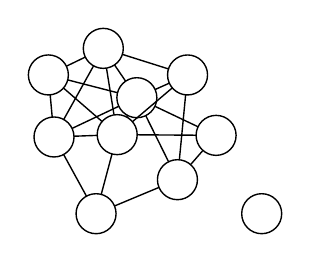
\begin{tikzpicture}[>=latex',line join=bevel,scale=.4]
  \pgfsetlinewidth{.5bp}
%%
\pgfsetcolor{black}
  % Edge: 5 -- 0
  \draw [] (50.975bp,158.84bp) .. controls (45.582bp,156.23bp) and (39.597bp,153.34bp)  .. (34.222bp,150.74bp);
  % Edge: 5 -- 1
  \draw [] (84.643bp,161.37bp) .. controls (96.964bp,157.48bp) and (113.5bp,152.27bp)  .. (125.86bp,148.36bp);
  % Edge: 6 -- 0
  \draw [] (21.443bp,105.03bp) .. controls (20.863bp,111.4bp) and (20.211bp,118.58bp)  .. (19.631bp,124.95bp);
  % Edge: 6 -- 2
  \draw [] (31.856bp,71.036bp) .. controls (37.972bp,59.88bp) and (46.093bp,45.065bp)  .. (52.198bp,33.928bp);
  % Edge: 6 -- 5
  \draw [] (31.841bp,102.81bp) .. controls (39.568bp,116.7bp) and (50.773bp,136.84bp)  .. (58.539bp,150.8bp);
  % Edge: 7 -- 1
  \draw [] (135.92bp,66.785bp) .. controls (137.53bp,83.477bp) and (139.91bp,108.08bp)  .. (141.51bp,124.75bp);
  % Edge: 7 -- 2
  \draw [] (117.55bp,41.664bp) .. controls (105.65bp,36.69bp) and (89.681bp,30.016bp)  .. (77.737bp,25.024bp);
  % Edge: 7 -- 3
  \draw [] (146.34bp,62.563bp) .. controls (149.79bp,66.518bp) and (153.54bp,70.819bp)  .. (156.97bp,74.761bp);
  % Edge: 8 -- 0
  \draw [] (79.976bp,126.94bp) .. controls (66.776bp,130.34bp) and (48.816bp,134.96bp)  .. (35.628bp,138.36bp);
  % Edge: 8 -- 1
  \draw [] (114.12bp,129.78bp) .. controls (118.2bp,131.62bp) and (122.58bp,133.58bp)  .. (126.67bp,135.42bp);
  % Edge: 8 -- 3
  \draw [] (114.19bp,114.53bp) .. controls (125.71bp,109.05bp) and (141.01bp,101.78bp)  .. (152.51bp,96.32bp);
  % Edge: 8 -- 5
  \draw [] (87.424bp,137.42bp) .. controls (84.273bp,142.05bp) and (80.806bp,147.15bp)  .. (77.657bp,151.78bp);
  % Edge: 8 -- 6
  \draw [] (81.103bp,114.54bp) .. controls (68.744bp,108.69bp) and (51.929bp,100.72bp)  .. (39.582bp,94.871bp);
  % Edge: 8 -- 7
  \draw [] (105.76bp,106.01bp) .. controls (111.81bp,93.786bp) and (120.04bp,77.152bp)  .. (126.09bp,64.937bp);
  % Edge: 9 -- 0
  \draw [] (66.194bp,101.08bp) .. controls (55.929bp,109.98bp) and (41.964bp,122.1bp)  .. (31.708bp,131.0bp);
  % Edge: 9 -- 1
  \draw [] (93.68bp,100.8bp) .. controls (104.16bp,109.69bp) and (118.53bp,121.89bp)  .. (129.11bp,130.87bp);
  % Edge: 9 -- 2
  \draw [] (75.241bp,71.56bp) .. controls (72.339bp,60.696bp) and (68.624bp,46.796bp)  .. (65.707bp,35.879bp);
  % Edge: 9 -- 3
  \draw [] (97.955bp,89.017bp) .. controls (113.3bp,88.906bp) and (135.24bp,88.748bp)  .. (150.67bp,88.636bp);
  % Edge: 9 -- 5
  \draw [] (77.041bp,107.16bp) .. controls (75.021bp,119.7bp) and (72.338bp,136.36bp)  .. (70.321bp,148.89bp);
  % Edge: 9 -- 6
  \draw [] (61.949bp,88.484bp) .. controls (55.311bp,88.239bp) and (47.792bp,87.962bp)  .. (41.147bp,87.717bp);
  % Edge: 9 -- 8
  \draw [] (88.59bp,105.38bp) .. controls (88.73bp,105.64bp) and (88.871bp,105.9bp)  .. (89.011bp,106.17bp);
  % Node: 0
\begin{scope}
  \definecolor{strokecol}{rgb}{0.0,0.0,0.0};
  \pgfsetstrokecolor{strokecol}
  \draw (18.0bp,142.9bp) ellipse (18.0bp and 18.0bp);
\end{scope}
  % Node: 1
\begin{scope}
  \definecolor{strokecol}{rgb}{0.0,0.0,0.0};
  \pgfsetstrokecolor{strokecol}
  \draw (143.26bp,142.87bp) ellipse (18.0bp and 18.0bp);
\end{scope}
  % Node: 2
\begin{scope}
  \definecolor{strokecol}{rgb}{0.0,0.0,0.0};
  \pgfsetstrokecolor{strokecol}
  \draw (60.93bp,18.0bp) ellipse (18.0bp and 18.0bp);
\end{scope}
  % Node: 3
\begin{scope}
  \definecolor{strokecol}{rgb}{0.0,0.0,0.0};
  \pgfsetstrokecolor{strokecol}
  \draw (168.96bp,88.5bp) ellipse (18.0bp and 18.0bp);
\end{scope}
  % Node: 4
\begin{scope}
  \definecolor{strokecol}{rgb}{0.0,0.0,0.0};
  \pgfsetstrokecolor{strokecol}
  \draw (210.0bp,18.0bp) ellipse (18.0bp and 18.0bp);
\end{scope}
  % Node: 5
\begin{scope}
  \definecolor{strokecol}{rgb}{0.0,0.0,0.0};
  \pgfsetstrokecolor{strokecol}
  \draw (67.44bp,166.8bp) ellipse (18.0bp and 18.0bp);
\end{scope}
  % Node: 6
\begin{scope}
  \definecolor{strokecol}{rgb}{0.0,0.0,0.0};
  \pgfsetstrokecolor{strokecol}
  \draw (23.08bp,87.05bp) ellipse (18.0bp and 18.0bp);
\end{scope}
  % Node: 7
\begin{scope}
  \definecolor{strokecol}{rgb}{0.0,0.0,0.0};
  \pgfsetstrokecolor{strokecol}
  \draw (134.17bp,48.61bp) ellipse (18.0bp and 18.0bp);
\end{scope}
  % Node: 8
\begin{scope}
  \definecolor{strokecol}{rgb}{0.0,0.0,0.0};
  \pgfsetstrokecolor{strokecol}
  \draw (97.65bp,122.39bp) ellipse (18.0bp and 18.0bp);
\end{scope}
  % Node: 9
\begin{scope}
  \definecolor{strokecol}{rgb}{0.0,0.0,0.0};
  \pgfsetstrokecolor{strokecol}
  \draw (79.94bp,89.15bp) ellipse (18.0bp and 18.0bp);
\end{scope}
%
\end{tikzpicture}
\caption{Minimal induced universal graphs for the families of all
graphs with 3, 4, and 5 vertices}
\label{fig:graphs}
\end{figure}

\section{\texorpdfstring{$f(6) = 14$}{f(6)=14}}\label{sec:f6}

This section shows that $f(6) = 14$.  We begin with the lower bound.
For $k \geq 6$, we can increase by 2 the lower bound by ``bof''.  In particular,
this means that $f(6) \geq 14$.

\begin{proposition}\label{f6proposition}
    $f(k) \geq 2k + 2$ for all $k \geq 6$.
\end{proposition}
\begin{proof}

    Suppose that $G$ is an induced universal graph for the family of all graphs
    on $k$ vertices, and that $G$ has no more than $2k + 1$ vertices.  Graph
    $G$ must have $K_k$ and $I_k$ as induced sugraphs.  This clique and
    independent set may overlap by no more than one vertex, so their union must
    contain at least $2k - 1$ vertices.  Therefore it is possible to partition
    the vertices of $G$ into three sets: a clique $S_1$, an independent set
    $S_2$, and a third set $S_3$ containing at most 2 vertices.

    We will show that $G$ cannot contain as induced subgraphs both
    of the graphs in Figure~\ref{fig:boundproof}.  These graphs are complements
    of each other, and we refer to them as $H$ and $H'$ respectively.

\begin{figure}[htb]
    \centering

% \begin{tikzpicture}[>=latex',line join=bevel]
%   \tikzstyle{every node}=[draw, circle, inner sep=1pt, minimum size=.5cm]
%   \pgfsetlinewidth{.5bp}
%   \node at (0,2.9) (1) {};
%   \node at (0,2) (2) {};
%   \node at (0,1.1) (3) {};
%   \node at (1.1,2.9) (4) {};
%   \node at (1.1,2) (5) {};
%   \node at (1.1,1.1) (6) {};
%   \draw (1) -- (2) -- (3);
%   \draw (3) to [out=140,in=220] (1);
%   \draw (4) -- (5) -- (6);
%   \draw (6) to [out=40,in=-40] (4);
%   \draw (1) -- (4);
%   \draw (1) -- (5);
%   \draw (1) -- (6);
%   \draw (2) -- (4);
%   \draw (2) -- (5);
%   \draw (2) -- (6);
%   \draw (3) -- (4);
%   \draw (3) -- (5);
%   \draw (3) -- (6);
% \end{tikzpicture}
% \qquad \qquad
% \begin{tikzpicture}
%   \tikzstyle{every node}=[draw, circle, inner sep=1pt, minimum size=.5cm]
%   \pgfsetlinewidth{.5bp}
%   \node at (0,2.9) (1) {};
%   \node at (0,2) (2) {};
%   \node at (0,1.1) (3) {};
%   \node at (1.1,2.9) (4) {};
%   \node at (1.1,2) (5) {};
%   \node at (1.1,1.1) (6) {};
% \end{tikzpicture}
% \qquad \qquad
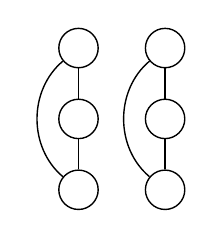
\begin{tikzpicture}[>=latex',line join=bevel]
  \tikzstyle{every node}=[draw, circle, inner sep=1pt, minimum size=.5cm]
  \pgfsetlinewidth{.5bp}
  \node at (0,2.9) (1) {};
  \node at (0,2) (2) {};
  \node at (0,1.1) (3) {};
  \node at (1.1,2.9) (4) {};
  \node at (1.1,2) (5) {};
  \node at (1.1,1.1) (6) {};
  \draw (1) -- (2) -- (3);
  \draw (3) to [out=140,in=220] (1);
  \draw (4) -- (5) -- (6);
  \draw (6) to [out=140,in=220] (4);
\end{tikzpicture}
\qquad \qquad
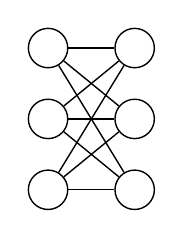
\begin{tikzpicture}[>=latex',line join=bevel]
  \tikzstyle{every node}=[draw, circle, inner sep=1pt, minimum size=.5cm]
  \pgfsetlinewidth{.5bp}
  \node at (0,2.9) (1) {};
  \node at (0,2) (2) {};
  \node at (0,1.1) (3) {};
  \node at (1.1,2.9) (4) {};
  \node at (1.1,2) (5) {};
  \node at (1.1,1.1) (6) {};
  \draw (1) -- (4);
  \draw (1) -- (5);
  \draw (1) -- (6);
  \draw (2) -- (4);
  \draw (2) -- (5);
  \draw (2) -- (6);
  \draw (3) -- (4);
  \draw (3) -- (5);
  \draw (3) -- (6);
\end{tikzpicture}
%%
\caption{If $k > 5$ and $G$ is a graph on $2k + 1$ or fewer vertices, then
$G$ cannot have as induced subgraphs all four of the following graphs: the
clique $K_k$, the independent set $I_k$, and
the two graphs shown. See the the proof of Proposition~\ref{f6proposition}}.
\label{fig:boundproof}
\end{figure}

    Let $G_1$ be an induced
    subgraph of $G$ that is isomorphic to $H$.  Since there are
    no edges between the two three-vertex cliques in $G_1$, it must be the case that the
    vertex set of at least one of these cliques does not intersect $S_1$.
    Since $S_2$ is an independent set in $G$, this clique must have exactly
    one vertex in $S_2$ and two vertices in $S_3$.  We can deduce, then, that
    $S_3$ contains exactly two vertices, and that these vertices are adjacent in $G$.

    Now consider graph $H'$.  Since $H'$ is an induced subgraph of $G$, it
    follows by taking complements of $H'$ and $G$ that $H$ is an induced
    subgraph of $G'$ (the complement of $G$).  We can repeat the argument
    of the previous paragraph with the roles of $S_1$ and $S_2$ reversed to
    show that the two vertices in $S_3$ must be adjacent in the complement of
    $G$, and therefore must not be adjacent in $G$.  Since we previously showed that
    these vertices are adjacent in $G$, we have a contradiction.
\end{proof}

To give an upper bound of 14 on $f(6)$, Figure~\ref{fig:adjmat14} shows the
adjacency matrix of a 14-vertex graph that is induced universal for the family
of all graphs on six vertices.  This was generated using a simple local search
algorithm.  We begin by generating a random graph on 14 vertices as follows.
We number the vertices from zero; the generator makes the
$k$ vertices numbered $0$ to $k-1$ a clique, and the $k$ vertices numbered $k-1$ to $2k-2$ an
independent set.\footnote{The clique and the independent set thus have one vertex
in common.  The proof of Proposition~\ref{f6proposition} can be modified straightforwardly
to show that there is no 14-vertex induced universal graph for this family of graphs
that contains a 6-vertex clique and a 6-vertex independent set as
induced subgraphs with disjoint vertex sets.}
Each possible edge that is not involved in either the clique
or the independent set is added with probability $1/2$.
We then repeatedly ``flip'' the status of a random edge from present to absent
or vice versa, but always leave the large clique and independent set intact.
After each flip, we count the number of 156 graphs on 6 vertices that are isomorphic
to a subgraph of our 14-vertex graph.  If the most recent flip decreased
this number, we revert it.  After each 1000 flips, we restart the algorithm
with a new random graph.

\begin{figure}[htb]
\centering
\small
\verb|0 1 1 1 1 1 0 1 1 0 0 0 1 0| \\
\verb|1 0 1 1 1 1 1 1 1 1 1 0 0 1| \\
\verb|1 1 0 1 1 1 0 1 1 0 1 0 1 0| \\
\verb|1 1 1 0 1 1 1 0 0 0 1 1 0 0| \\
\verb|1 1 1 1 0 1 0 1 0 0 0 0 0 0| \\
\verb|1 1 1 1 1 0 0 0 0 0 0 1 0 1| \\
\verb|0 1 0 1 0 0 0 0 0 0 0 1 1 1| \\
\verb|1 1 1 0 1 0 0 0 0 0 0 1 1 0| \\
\verb|1 1 1 0 0 0 0 0 0 0 0 0 1 0| \\
\verb|0 1 0 0 0 0 0 0 0 0 0 1 0 1| \\
\verb|0 1 1 1 0 0 0 0 0 0 0 1 1 0| \\
\verb|0 0 0 1 0 1 1 1 0 1 1 0 0 1| \\
\verb|1 0 1 0 0 0 1 1 1 0 1 0 0 0| \\
\verb|0 1 0 0 0 1 1 0 0 1 0 1 0 0|
\caption{The adjacency matrix of a 14-vertex induced universal graph for the family of all
six-vertex graphs}
\label{fig:adjmat14}
\end{figure}

\section{Bounds on \texorpdfstring{$f(7)$}{f(7)}}\label{sec:f7}

By Proposition~\ref{f6proposition}, we have $f(7) \geq 16$.  Figure~\ref{fig:adjmat18}
shows the adjacency matrix of an 18-vertex induced universal
graph for the family of all seven-vertex graphs. This was generated with 
the heuristic described in Section~\ref{sec:f6}, with two modifications.
First, 10000 rather than 1000
edge-flips were permitted before each restart, as this was found to be more effective
in a preliminary run of the experiment.  Second, the overlapping six-vertex clique
and independent set were replaced with a clique on seven vertices and an independent
set on seven vertices.  Again, these had one vertex in common.  (We also tried making
the clique and independent set vertex-disjoint, but did not find an 18-vertex solution
in four hours with this approach.)

Thus we have $16 \leq f(7) \leq 18$.

\begin{figure}[htb]
\centering
\small
\verb|0 1 1 1 1 1 1 1 1 1 0 1 1 1 1 1 0 0| \\
\verb|1 0 1 1 1 1 1 0 1 1 1 0 1 1 0 1 0 0| \\
\verb|1 1 0 1 1 1 1 1 0 1 0 1 0 0 0 0 0 1| \\
\verb|1 1 1 0 1 1 1 0 1 0 0 1 0 0 0 0 0 1| \\
\verb|1 1 1 1 0 1 1 1 1 0 0 0 0 0 1 0 0 0| \\
\verb|1 1 1 1 1 0 1 0 1 0 0 0 0 1 1 1 1 1| \\
\verb|1 1 1 1 1 1 0 0 0 0 0 0 0 1 0 0 0 1| \\
\verb|1 0 1 0 1 0 0 0 0 0 0 0 0 0 1 1 1 0| \\
\verb|1 1 0 1 1 1 0 0 0 0 0 0 0 1 1 1 0 1| \\
\verb|1 1 1 0 0 0 0 0 0 0 0 0 0 0 1 1 1 1| \\
\verb|0 1 0 0 0 0 0 0 0 0 0 0 0 1 0 0 1 0| \\
\verb|1 0 1 1 0 0 0 0 0 0 0 0 0 0 1 1 1 0| \\
\verb|1 1 0 0 0 0 0 0 0 0 0 0 0 0 0 1 1 1| \\
\verb|1 1 0 0 0 1 1 0 1 0 1 0 0 0 0 0 0 1| \\
\verb|1 0 0 0 1 1 0 1 1 1 0 1 0 0 0 0 0 1| \\
\verb|1 1 0 0 0 1 0 1 1 1 0 1 1 0 0 0 1 1| \\
\verb|0 0 0 0 0 1 0 1 0 1 1 1 1 0 0 1 0 1| \\
\verb|0 0 1 1 0 1 1 0 1 1 0 0 1 1 1 1 1 0|
\caption{The adjacency matrix of an 18-vertex induced universal graph for the family of all
seven-vertex graphs}
\label{fig:adjmat18}
\end{figure}

\section{Trees}\label{sec:trees}

Table~\ref{tab:treeresults} gives the order $t(k)$ of a minimal induced universal graph for
the family of $k$-vertex trees, and the number $T(k)$ of such graphs.  Figure~\ref{fig:trees}
shows one of the 66 minimal induced universal graphs for the family of 6-vertex trees.

\section{Acknowledgements}

I would like to thank Brendan McKay for helpful feedback on this paper, and Persi
Diaconis for introducing me to induced universal graphs and for interesting email
discussions on related topics.

\begin{table}[h!]
\centering
\begin{tabular}{r r r}
 \toprule
 $k$ & $t(k)$ & $T(k)$ \\ [0.5ex]
 \midrule
 1 & 1 & 1 \\
 2 & 2 & 1 \\
 3 & 3 & 1 \\
 4 & 5 & 2 \\
 5 & 7 & 18 \\
 6 & 9 & 66 \\
 \bottomrule
\end{tabular}
\caption{For each $k$, $t(k)$ is the minimum order of a graph containing all $k$-vertex trees as
induced subgraphs, and $T(k)$ is the number of distinct $t(k)$-vertex graphs that contain
all $k$-vertex trees as induced subgraphs.}
\label{tab:treeresults}
\end{table}

\begin{figure}[htb]
    \centering
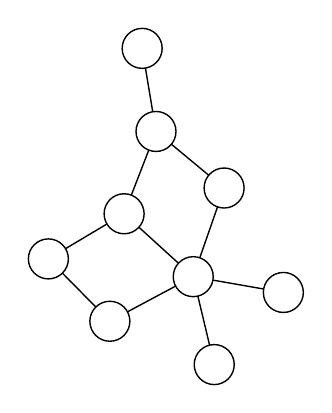
\begin{tikzpicture}[>=latex',line join=bevel,scale=.4]
  \pgfsetlinewidth{.5bp}
%%
\pgfsetcolor{black}
  % Edge: 6 -- 0
  \draw [] (33.468bp,122.33bp) .. controls (44.467bp,128.89bp) and (59.197bp,137.66bp)  .. (70.288bp,144.27bp);
  % Edge: 6 -- 1
  \draw [] (30.834bp,100.1bp) .. controls (39.774bp,91.035bp) and (51.646bp,78.993bp)  .. (60.571bp,69.941bp);
  % Edge: 7 -- 0
  \draw [] (108.35bp,211.0bp) .. controls (103.69bp,198.96bp) and (97.434bp,182.81bp)  .. (92.754bp,170.73bp);
  % Edge: 7 -- 2
  \draw [] (128.78bp,216.26bp) .. controls (138.81bp,207.93bp) and (152.29bp,196.74bp)  .. (162.31bp,188.42bp);
  % Edge: 7 -- 3
  \draw [] (111.85bp,245.92bp) .. controls (109.9bp,257.68bp) and (107.35bp,272.94bp)  .. (105.4bp,284.67bp);
  % Edge: 8 -- 0
  \draw [] (134.88bp,109.4bp) .. controls (124.44bp,118.9bp) and (110.07bp,131.98bp)  .. (99.64bp,141.47bp);
  % Edge: 8 -- 1
  \draw [] (132.46bp,88.608bp) .. controls (119.73bp,81.799bp) and (101.96bp,72.297bp)  .. (89.227bp,65.491bp);
  % Edge: 8 -- 2
  \draw [] (154.41bp,114.43bp) .. controls (159.1bp,127.91bp) and (165.58bp,146.51bp)  .. (170.24bp,159.91bp);
  % Edge: 8 -- 4
  \draw [] (166.38bp,93.965bp) .. controls (179.82bp,91.611bp) and (198.11bp,88.409bp)  .. (211.53bp,86.058bp);
  % Edge: 8 -- 5
  \draw [] (152.57bp,79.558bp) .. controls (155.7bp,66.447bp) and (159.96bp,48.609bp)  .. (163.09bp,35.509bp);
  % Node: 0
\begin{scope}
  \definecolor{strokecol}{rgb}{0.0,0.0,0.0};
  \pgfsetstrokecolor{strokecol}
  \draw (86.17bp,153.73bp) ellipse (18.0bp and 18.0bp);
\end{scope}
  % Node: 1
\begin{scope}
  \definecolor{strokecol}{rgb}{0.0,0.0,0.0};
  \pgfsetstrokecolor{strokecol}
  \draw (73.34bp,56.99bp) ellipse (18.0bp and 18.0bp);
\end{scope}
  % Node: 2
\begin{scope}
  \definecolor{strokecol}{rgb}{0.0,0.0,0.0};
  \pgfsetstrokecolor{strokecol}
  \draw (176.16bp,176.91bp) ellipse (18.0bp and 18.0bp);
\end{scope}
  % Node: 3
\begin{scope}
  \definecolor{strokecol}{rgb}{0.0,0.0,0.0};
  \pgfsetstrokecolor{strokecol}
  \draw (102.42bp,302.6bp) ellipse (18.0bp and 18.0bp);
\end{scope}
  % Node: 4
\begin{scope}
  \definecolor{strokecol}{rgb}{0.0,0.0,0.0};
  \pgfsetstrokecolor{strokecol}
  \draw (229.48bp,82.92bp) ellipse (18.0bp and 18.0bp);
\end{scope}
  % Node: 5
\begin{scope}
  \definecolor{strokecol}{rgb}{0.0,0.0,0.0};
  \pgfsetstrokecolor{strokecol}
  \draw (167.27bp,18.0bp) ellipse (18.0bp and 18.0bp);
\end{scope}
  % Node: 6
\begin{scope}
  \definecolor{strokecol}{rgb}{0.0,0.0,0.0};
  \pgfsetstrokecolor{strokecol}
  \draw (18.0bp,113.12bp) ellipse (18.0bp and 18.0bp);
\end{scope}
  % Node: 7
\begin{scope}
  \definecolor{strokecol}{rgb}{0.0,0.0,0.0};
  \pgfsetstrokecolor{strokecol}
  \draw (114.87bp,227.81bp) ellipse (18.0bp and 18.0bp);
\end{scope}
  % Node: 8
\begin{scope}
  \definecolor{strokecol}{rgb}{0.0,0.0,0.0};
  \pgfsetstrokecolor{strokecol}
  \draw (148.38bp,97.12bp) ellipse (18.0bp and 18.0bp);
\end{scope}
%
\end{tikzpicture}

\caption{A universal graph for the family of all
trees with 6 vertices}
\label{fig:trees}
\end{figure}

\bibliographystyle{abbrv}
\bibliography{main}
%
\end{document}
%



